\documentclass[parskip=full]{scrartcl}

\pdfoutput=1

\title{Tabular synthetic data generation: A literature review}

\author{%
	Joao Fonseca\(^{1*}\), Fernando Bacao\(^{1}\)
	\\
	\small{\(^{1}\)NOVA Information Management School, Universidade Nova de Lisboa}
	\\
	\small{*Corresponding Author}
	\\
	\\
	\small{Postal Address: NOVA Information Management School, Campus de
    Campolide, 1070--312 Lisboa, Portugal}
	\\
	\small{Telephone: +351 21 382 8610}
}

\usepackage{float}
\usepackage{graphicx}
\usepackage{geometry}
\geometry{%
	a4paper,
	left=18mm,
	right=18mm,
	top=18mm,
}
\usepackage{amsmath}
\usepackage{amsfonts}
\usepackage{enumitem}
\usepackage[ruled,vlined]{algorithm2e}
\usepackage{booktabs}
\usepackage{pgfplotstable}
\pgfplotsset{compat=1.14}
\usepackage{longtable}
\usepackage{tabu}
\usepackage{hyperref}
\usepackage{lineno}
\date{}


% use \citet for inline text references, \cite for normal citations
\usepackage[
    style=numeric,
    citestyle=numeric,
    sorting=none,
    natbib=true,
    backend=biber, 
    maxcitenames=1, 
    maxbibnames=99
]{biblatex}
\bibliography{references}
\usepackage{breakcites}

% Fix underfull hbox warnings in bilbliography
% Reference: https://tex.stackexchange.com/questions/10924/underfull-hbox-in-bibliography
\usepackage{etoolbox}
\apptocmd{\sloppy}{%
    \hbadness%
    10000\relax
}{}{}

% Fix overfull hbox warnings in bibliography
% Reference: https://tex.stackexchange.com/questions/171999/overfull-hbox-in-biblatex
\usepackage[T1]{fontenc}
\usepackage[final]{microtype}

% Highlight text: \hl
\usepackage{soul}

\definecolor{hypecol}{HTML}{0875b7}
\hypersetup{%
    colorlinks,
    linkcolor={hypecol},
    citecolor={hypecol},
    urlcolor={hypecol}
}

% Case-dependent packages here
\usepackage{tabularx}
\renewcommand\tabularxcolumn[1]{m{#1}}% for vertical centering text in X column

\begin{document}

\maketitle
\linenumbers

\begin{abstract}

    The generation of synthetic data can be used for anonymization,
    regularization, oversampling, semi-supervised learning, self-supervised
    learning and various other tasks. The wide range of applications of these
    mechanisms motivated the development of new algorithms specialized in
    generating data for specific types of data and Machine Learning (ML)
    tasks. As a result, the analysis of the different types of generative
    models 

    % We provide a broad taxonomy to define data generation mechanisms

    % We provide an analysis on recommendations for the evaluation of the
    % quality of the synthetic data generated

\end{abstract}

\section{Introduction}\label{sec:introduction}

Synthetic data is obtained from a generative process based on properties of
real data~\cite{assefa2020generating}. The generation of synthetic data is
essential for various domains and tasks. For example, synthetic data is used
as a form of regularizing neural networks (\textit{i.e.}, data augmentation)
\textbf{[CITATION]}. One form of anonymizing datasets is via the production of
synthetic observations (\textit{i.e.}, synthetic data generation)
\textbf{[CITATION]}. In settings where only a small portion of training data
is labeled, some techniques generate artificial data using both labeled and
unlabeled data with a modified loss function to train neural networks
(\textit{i.e.}, semi-supervised learning)~\cite{laine2017temporal}. In
imbalanced learning contexts, synthetic data can be used to balance the target
classes' frequencies and reinforce the learning of minority classes
(\textit{i.e.}, oversampling)~\cite{fonseca2021improving}. Some active
learning frameworks use data generation to improve the quality of data
selection and classifier training~\cite{kim2021lada}. Other techniques employ
data generation to produce deep neural networks without labeled data
(\textit{i.e.}, self-supervised learning)~\cite{grill2020bootstrap}.

% TODO: Use this as inspiration to further justify the need for this literature
% review:
%
% These methods heavily rely on the unique structure in the domain datasets
% (such as spatial relationships in images or semantic relationships in
% language). They are not adaptable to general tabular data which does not
% have the same explicit structure as image and language data.
%
%
% Own authorship:
%
% Data generation techniques in tabular data settings are not as explored as
% in image or text formats, depite its popularity and
% ubiquity~\cite{fakoor2020fast}.

The breadth of these techniques span multiple domains, such as facial
recognition~\cite{lv2017data}, Land Use/Land Cover mapping
\textbf{[CITATION]}, medical image processing \textbf{[CITATION]}, Natural
Language Processing (NLP)~\cite{feng2021survey} or credit card default
prediction~\cite{alam2020investigation}. According to the domain and data
type, the data generation techniques used may vary significantly. Generally
speaking, some data generation mechanisms are specific to some domains, data
types or tasks. \hl{For example, \ldots}. Most, if not all, of these
techniques are applied on the input or output space.

However, there are various data generation techniques that are invariant to
the task or data types used. These techniques can be either applied in the
feature space~\cite{devries2017dataset} or in tabular
datasets\footnote{Tabular data is a database structured in tabular form,
composed of columns (features) and rows (observations)~\cite{yoon2020vime}}.
On one hand, data generation in the feature space uses a generative model to
learn a manifold, lower-dimensional abstraction over the input
space~\cite{kingma2019introduction}, defined here as the feature space. At
this level, any tabular data generation mechanism can be applied and
reconstructed into the input space if necessary. On the other hand, synthetic
data generation on tabular data can be applied to most problems. Although, the
choice of generation mechanism is still dependant on (1) the importance of the
relationships found between the different features, (2) the ML task developed
and (3) the motivation for the generation of synthetic data. For example, when
generating data to address an imbalanced learning problem (\textit{i.e.},
oversampling), the relationships between the different features are not
necessarily kept since the goal is to reinforce the learning of the minority
class by redefining an ML classifier's decision boundaries. If the goal is to
anonymize a dataset, perform some type of descriptive task, or ensure a
consistent model interpretability, these relationships need to be kept.

Depending on the context, evaluating the quality of the generated data is a
complex task. For example, for image and time series data, perceptually small
changes in the original data can lead to large changes in the euclidean
distance~\cite{assefa2020generating, theis2016note}. The evaluation of
generative models typically account primarily for the performance in a
specific task, since good performance in one criterion does not imply good
performance on another~\cite{theis2016note}. However, in computationally
intensive tasks it is often impracticable to search for the optimal
configurations of generative models. To address this limitation, other
evaluation methods have been proposed to assist in this evaluation, which can
be distinguished into statistical divergence metrics and precision/recall
metrics~\cite{alaa2022faithful}. The relevant performance metrics found in the
literature are discussed in Section~\ref{sec:evaluating-synthetic-data}.

% Discuss Generative models -> Network based models

\subsection{Motivation, Scope and Contributions}

% TODO: Define scope
% - Exclude domain-specific traditional applications
% - Exclude Generation techniques with an internal application level
% - Preference for methods published in 2019 or later, 
%   non-traditional methods, or unique/uncommon approaches
% - To avoid redundancy, this is a non-comprehensive analysis of algorithms
%   and problems using synthetic data. Instead, we show the most important
%   methods using each of the data generation mechanisms found. For example,
%   there are several oversampling algorithms available, but most of those
%   excluded from this analysis use a linear (SMOTE-based) generation
%   mechanism.

This literature review focuses on generation mechanisms applied to tabular
data and the different ML techniques where tabular synthetic data is used. In
addition, we focus on the ML perspective of synthetic data, as opposed to the
practical perspective. From a practical sense, synthetic data is used as a
proxy of real data. It is assumed to be inaccessible, essential and a
secondary asset for tasks like education, software development, or systems
demonstrations~\cite{mannino2019real}. 

We focus on data generation techniques in the tabular and feature space
(\textit{i.e.}, embedded inputs), given its breadth in scope. Related
literature reviews are mostly focused on specific algorithmic or domain
applications, with little to no emphasis on the core generative process. For
this reason, these techniques often appear ``sandboxed'', even though there is
a significant overlap between them. There are some related reviews published
since 2019. \citet{assefa2020generating} provides a general overview of
synthetic data generation for time series data anonymization in the finance
sector. \citet{hernandez2022synthetic} reviews data generation techniques for
tabular health records anonymization. \citet{raghunathan2021synthetic} reviews
synthetic data anonymization techniques that preserve the statistical
properties of a dataset. \citet{nalepa2019data} reviews data augmentation
techniques for brain-tumor segmentation. \citet{bayer2021survey} distinguishes
augmentation techniques for text classification into feature and data space,
while providing an extensive overview of augmentation methods within this
domain. However, the taxonomy proposed and feature space augmentation methods
are not necessarily specific to the domain. \citet{shorten2021text},
\citet{chen2021empirical}, \citet{feng2021survey} and \citet{liu2020survey}
also review data augmentation techniques for text data.
\citet{yi2019generative} review Generative Adversarial Network architectures
for medical imaging. \citet{wang2020survey} reviews face data augmentation
techniques. \citet{shorten2019survey} and \citet{khosla2020enhancing} discuss
techniques for image data augmentation. \citet{iwana2021empirical} and
\citet{wen2020time} also review time series data augmentation techniques.
\citet{zhao2022graph} review data augmentation techniques for graph data. The
analysis of related literature reviews~\footnote{%
    Results obtained using Google Scholar, limited to articles published since
    2019, using the search query {\fontfamily{qcr}\selectfont (``synthetic
    data generation'' OR ``oversampling'' OR ``imbalanced learning'' OR ``data
    augmentation'') AND (``literature review'' OR ``survey'')}. Retrieved on
    August $11^{th}$, 2022. More articles were added later whenever found
    relevant.
} is shown in Table~\ref{tab:literature-reviews}.

% TODO: move table to appendix (?)
\begin{table}[t!]
    \centering
    \caption{\label{tab:literature-reviews}
        Related literature reviews published since 2019.
    }
    \small{%
    \begin{tabularx}{\textwidth}{@{}rcccX@{}}
        \toprule
        Reference & Data type & ML problem & Domain & Observations \\
        \midrule

        \citet{assefa2020generating} & --- & Differential privacy &
        Finance & Analysis of applications, motivation and properties of
        synthetic data for anonymization. \\

        \citet{hernandez2022synthetic} & Tabular & Differential privacy &
        Healthcare & Focus on GANs. \\

        \citet{raghunathan2021synthetic} & Tabular & Differential privacy &
        Statistics & Focus on general definitions such as differential privacy
        and statistical disclosure control.\\

        \citet{nalepa2019data} & Image & Segmentation & Medicine & Analysis of
        algorithmic applications on a 2018 brain-tumor segmentation
        challenge.\\

        \citet{bayer2021survey} & Text & Classification & --- & Distinguish
        100 methods into 12 groups. \\

        \citet{shorten2021text} & Text & Deep Learning & --- & General
        overview of text data augmentation. \\

        \citet{chen2021empirical} & Text & Few-shot Learning & --- &
        Augmentation techniques for machine learning with limited data\\

        \citet{feng2021survey} & Text & --- & --- & Overview of augmentation
        techniques and applications on NLP tasks.\\

        \citet{liu2020survey} & Text & --- & Various & Analysis of industry
        use cases of data augmentation in NLP\@. Emphasis on input level data
        augmentation.\\

        \citet{yi2019generative} & Image & --- & Medicine & Emphasis on GANs.\\

        \citet{wang2020survey} & Image & Deep Learning & --- & Regularization
        techniques using facial image data. Emphasis on Deep Learning
        generative models.\\

        \citet{shorten2019survey} & Image & Deep Learning & --- & Emphasis on
        data augmentation as a regularization technique.\\

        \citet{khosla2020enhancing} & Image & --- & --- & Broad overview of
        image data augmentation. Emphasis on traditional approaches. \\

        \citet{iwana2021empirical} & Time series & Classification & --- &
        Defined a taxonomy for time series data augmentation.\\

        \citet{wen2020time} & Time series & Various & --- & Analysis of data
        augmentation methods for classification, anomaly detection and
        forecasting.\\

        \citet{zhao2022graph} & Graph & Various & --- & Graph data
        augmentation for supervised and self-supervised learning.\\

        \citet{khalifa2021comprehensive} & Image & --- & Various & General
        overview of image data augmentation and relevant domains of
        application.\\

        \bottomrule
        
    \end{tabularx}
    }
\end{table}


The different taxonomies established in the literature follow a similar
philosophy, but vary in terminology and are often specific to the technique
discussed. Regardless, it is possible to establish a broader taxonomy without
giving up on specificity. This study provides a joint overview of the
different data generation approaches, domains and ML techniques where data
generation is being used, as well as a common taxonomy across domains. It
extends the analyses found in these articles and uses the compiled knowledge
to identify research gaps. We compare the strengths and weaknesses of the
models developed within each of these fields. Finally, we identify possible
future research directions to address some of the limitations found. The
contributions of this paper are summarized below:

\begin{itemize}
    \item Bridge different ML concepts using synthetic data generation in its
        core \hl{(Algorithmic applications + Review of the State-of-the-art)}.
    \item Propose a synthetic data generation/data augmentation taxonomy to
        resolve the ambiguity in the literature \hl{(Data augmentation
        taxonomy)}.
    \item Characterize all relevant data generation methods using the proposed
        taxonomy. 
    \item Discuss the ML techniques in which synthetic data generation/data
        augmentation is used, beyond regularization and consolidate the
        current data generation mechanisms across the different techniques
        \hl{(Algorithmic Applications)}.
    \item Bring to light the key challenges of synthetic data generation and
        put forward possible research directions in the future.
\end{itemize}

% TODO: Develop research questions

\subsection{Paper Organization}

This paper is organized as follows: Section~\ref{sec:background} defines and
formalizes the different concepts, goals, trade-offs and motivations related
to synthetic data generation. Section~\ref{sec:taxonomy} establishes the
taxonomy used to categorize all the methods described in the paper.
Section~\ref{sec:feature-space} reviews synthetic data generation
mechanisms in the feature space. Section~\ref{sec:input-space}
reviews synthetic data generation mechanisms in the input space.
Section~\ref{sec:algorithmic-applications} describes the applications of
synthetic data in ML methods. Section~\ref{sec:evaluating-synthetic-data}
reviews performance evaluation methods of synthetic data generation
mechanisms. Section~\ref{sec:discussion} summarizes the main findings and
discusses limitations and possible research directions in the
state-of-the-art. Section~\ref{sec:conclusions} presents the main conclusions
drawn from this study.

\section{Background}\label{sec:background}

% Definition
In this section we define basics concepts, common goals, trade-offs and
motivations regarding the generation of synthetic data in ML\@. We define
synthetic data generation as the production of observations using a generative
model (regardless of its nature) that resemble naturally occurring
observations within a certain domain. It requires access to either a training
dataset, a generative process, or a data stream. However, additional
requirements might be imposed depending on the ML task being developed. For
example, to generate artificial data for regularization purposes in supervised
learning (\textit{i.e.}, data augmentation) the training dataset must be
annotated \textbf{[CITATION]}. The generation of synthetic data for
anonymization purposes assumes synthetic datasets to be different from the
original data, while following the same statistical properties
\textbf{[CITATION]}. Domain knowledge may also be necessary to encode specific
relationships among features into the generative process.


\subsection{Relevant Learning Problems}

%% Anonymize datasets (differential privacy)
The breach of sensitive information is an important barrier to the sharing of
datasets, especially when it concerns personal
information~\cite{dankar2021fake}. A common solution for this problem is the
generation of synthetic data without identifiable information. Generally
speaking, ML tasks that require data with sensitive information are not
compromised when using synthetic data. The experiment conducted by
\citet{patki2016synthetic} using relational datasets showed that in 11 out 15
comparisons ($\approx 73\%$), practitioners performing predictive modelling
tasks using fully synthetic datasets performed the same or better than those
using the original dataset. This topic is discussed in
Section~\ref{sec:data-privacy}.

%% Generalization/regularization
A common problem in the training of deep neural networks are their capacity to
generalize~\cite{Zhang2021} (\textit{i.e.}, reduce the difference in
classification performance between known and unseen observations). Data
augmentation is a common method to address this problem. The generation of
synthetic observations increases the range of the possible input space used in
the training phase, which reduces the performance difference between known and
unseen observations. Although other regularization methods exist, data
augmentation is a useful method since it does not affect the choice in the
architecture of the ML classifier and does not exclude the usage of other
regularization methods. In domains such as computer vision and NLP, data
augmentation is also used to improve the robustness of models against
adversarial attacks~\cite{zeng2020data, morris2020textattack}. These topics
are discussed into higher detail in Section~\ref{sec:regularization}.

%% Oversampling
In supervised learning, synthetic data generation is often motivated by the
need to balance target class distributions (\textit{i.e.}, oversampling).
Since most ML classifiers are designed to perform best with balanced datasets,
defining an appropriate decision boundary to distinguish rare classes becomes
difficult~\cite{saez2016analyzing}. Although there are other approaches to
address imbalanced learning, oversampling techniques are generally easier to
implement since they do not involve modifications to the classifier. This
topic is discussed into higher detail in Section~\ref{sec:oversampling}.

%% Active Learning + Few-shot Learning
In supervised learning projects where labeled data is not readily available,
but can be labeled, an Active Learning (AL) method may be used to improve the
labelling process. AL aims to reduce the cost of producing training datasets
by finding the most informative observations to label and feed into the
classifier~\cite{fonseca2021increasing}. In this case, the generation of
synthetic data is particularly useful to reduce the amount of labelled data
required for a successful ML project and its costs. A similar motivation
applies to the case of few-shot learning: small datasets may be expanded with
synthetic data~\cite{kumar2019closer}. These topics are discussed in
Sections~\ref{sec:active-learning} and~\ref{sec:few-shot-learning}.

%% Semi-supervised Learning + Self-supervised learning
The two other techniques reliant on synthetic data generation is 
Semi-supervised and Self-supervised learning. The former leverages both
labeled and unlabeled data in the training phase, simultaneously. Most of the
methods in the literature apply perturbations on the training data as part of
the training procedure~\cite{van2020survey}. Self-supervised learning is a
technique used to train neural networks in the absence of labeled data. Both
techniques use synthetic data generation as an internal procedure for most of
these methods. These techniques are discussed in
Sections~\ref{sec:semi-supervised-learning}
and~\ref{sec:self-supervised-learning}.


% Concepts definition, goals + trade-offs, Motivations

% Concepts definition
% - Original dataset
% - Synthetic dataset
% - Generator
% - Quality criteria (e.g., similarity function)
% - Objective performance metric (ML method to improve)
 
% Common success criteria 
% - The synthetic dataset should be different than the original dataset (i.e.,
%   no duplicates)
% - It should minimize a similarity function
% - The statistical properties of the dataset are preserved
% - It should improve the output of the objective performance
 
% Trade-offs
% - Additional computational overhead
% - Expose the classifier to unfeasible input areas

\subsection{Problem Formulation}\label{sec:problem-formulation}

The original dataset, $\mathcal{D} = \mathcal{D}_L \cup \mathcal{D}_U$,
is a collection of real observations and is distinguished according to whether
a target feature exists, $\mathcal{D}_L = {((x_i, y_i))}^l_{i=1}$, or not,
$\mathcal{D}_U = {(x_i)}^{u}_{i=1}$. All three datasets, $\mathcal{D}$,
$\mathcal{D}_L$ and $\mathcal{D}_U$ consist of ordered collections with
lengths $l+u$, $l$ and $u$, respectively. Synthetic data generation is
performed using a generator, $f_{gen}(x;\tau) = \tilde{x}$, where $\tau$
defines the generation policy (\textit{i.e.}, its hyperparameters), $x \in
\mathcal{D}$ is an observation and $\tilde{x} \in \mathcal{D}^s$ is a
synthetic observation. Analogous to $\mathcal{D}$, the synthetic dataset,
$\mathcal{D}^s$, is also distinguished according to whether there is an
assignment of a target feature, $\mathcal{D}^s_L = {((\tilde{x}_j,
\tilde{y}_j))}^{l'}_{j=1}$, or not, $\mathcal{D}^s_U =
{(\tilde{x}_j)}^{u'}_{j=1}$.

% - Quality criteria (e.g., similarity function)
Depending on the ML task, it may be relevant to establish metrics to measure
the quality of $\mathcal{D}^s$. In this case, a metric
$f_{qual}(\mathcal{D}^s, \mathcal{D})$ is used to determine the level of
similarity/dissimilarity between $\mathcal{D}$ and $\mathcal{D}^s$. In
addition, a performance metric to estimate the performance of a model on the
objective task, $f_{per}$, may be used to determine the appropriateness of a
model with parameters $\theta$, \textit{i.e.}, $f_{\theta}$. The generator's
goal is to generate $\mathcal{D}^s$ with arbitrary length, given
$\mathcal{D} \sim \mathbb{P}$ and $\mathcal{D}^s \sim \mathbb{P}^s$, such
that $\mathbb{P}^s \approx \mathbb{P}$, $x_i \neq x_j \forall x_i \in
\mathcal{D} \wedge x_j \in \mathcal{D}^s$. $f_{gen}(x;\tau)$ attempts to
generate a $\mathcal{D}^s$ that maximizes either $f_{per}$, $f_{qual}$, or a
combination of both.


\section{Data Generation Taxonomy}\label{sec:taxonomy}

The taxonomy proposed in this paper is a compilation of different definitions
found in the literature, along with other traits that vary among domains and
generation techniques. Within image data studies, \citet{shorten2019survey}
and \citet{khalifa2021comprehensive} divide data augmentation techniques into
``basic'' or ``classical'' approaches and deep learning approaches. In both
cases, the former refers to domain-specific generation techniques, while the
latter may be applied to any type of data. \citet{iwana2021empirical} proposes
a time-series data augmentation taxonomy divided in four families: (1)
Decomposition, (2) Pattern mixing, (3) Generative models and (4)
Decomposition. With exception to generative models, the majority of the
methods presented in the remaining families are well established and domain
specific. \citet{hernandez2022synthetic} defines a taxonomy for synthetic
tabular data generation approaches divided in three types of approaches: (1)
Classical, (2) Deep learning and (3) Others. Most taxonomies found followed
similar definitions with variations in terminology or distinction criteria. In
addition, all taxonomies with categories defined as ``basic'', ``traditional''
or ``classical'' use these to characterize domain-specific transformations.

Within the taxonomies found, none of them consider how a generation
mechanism employs $\mathcal{D}$ into the generation process or, if
applicable, the training phase. However, it is important to understand whether
a generation mechanism randomly selects $x$ and a set of close neighbors, thus
considering local information only, or considers the overall dataset or data
distribution for the selection of $x$ and/or generation of $\tilde{x}$. Our
proposed taxonomy is depicted in Figure~\ref{fig:data-generation-taxonomy}. It
characterizes data generation mechanisms using four properties:

\begin{enumerate}

    \item Architecture. Defines the broader type of data augmentation. It is
        based on domain specificity, architecture type or data transformations
        using a heuristic or random perturbation process. Generation
        techniques that apply a form of random perturbation, interpolation or
        geometric transformation to the data with some degree of randomness
        are considered randomized approaches. Typical, domain-specific data
        generation techniques are considered traditional architectures. These
        techniques apply transformations to a data point using \textit{a
        priori} domain knowledge. Generative models based on neural network
        architectures are defined as network-based. These architectures
        attempt to either generate observations in the feature space and/or by
        producing observations that are difficult to distinguish from the
        original dataset.

    \item Application level. Refers to the phase of the ML pipeline where the
        generative process is included. Generative models are considered
        internal if they are used alongside the primary ML task, whereas
        models used prior to the development of the primary ML task are
        considered external.

    \item Scope. Considers the usage of the original dataset's properties.
        Generative models that consider the density of the data space,
        statistical properties of $\mathcal{D}$, or attempt to replicate
        specific relationships found in $\mathcal{D}$ are considered to have
        a global scope, whereas generative models that consider a single
        observation and/or a set of close neighbors are considered to have a
        local scope. On the one hand, generative models with a local scope do
        not account for $\mathbb{P}^s$ but allow for a larger diversity of
        candidate $x^s$ and higher variance within $\mathcal{D}^s$. On the
        other hand, generative models with a global scope have a higher
        capacity to model $\mathbb{P}^s$ but produce candidate $x^s$ with
        lower diversity and lower variance within $\mathcal{D}^s$.

    \item Data space. Refers to the type data representation used to apply the
        generative model. Generation mechanisms can be applied using the raw
        dataset (\textit{i.e.}, on the input space), an embedded
        representation of the data (\textit{i.e.}, on the feature space) or
        based on the target feature (\textit{i.e.}, on the output space).
        Although some studies discuss the need to generate synthetic data on
        the input space~\cite{dankar2021fake, patki2016synthetic}, there are
        various studies that apply synthetic data generation techniques on a
        feature space.

\end{enumerate}

\begin{figure}
	\centering
	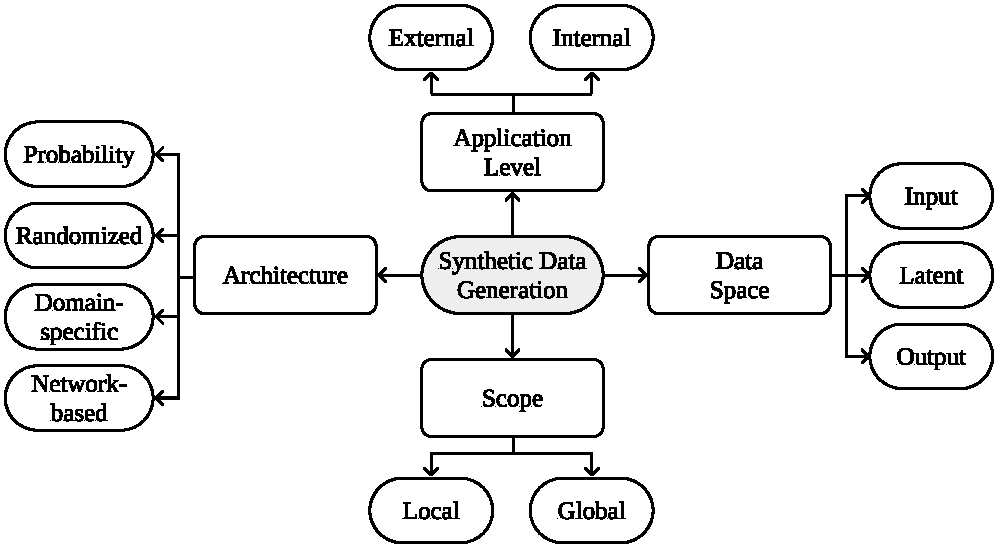
\includegraphics[width=.8\linewidth]{../analysis/data-generation-taxonomy}
    \caption{General taxonomy of data generation mechanisms proposed in this
        paper.
    }~\label{fig:data-generation-taxonomy}
\end{figure}

Throughout the analysis of the different types of generation mechanisms, all
relevant methods were characterized using this taxonomy and listed in
Table~\ref{tbl:generators}.

\begingroup\small
\begin{longtable}{rcccccccc}
    \caption{Summary of the synthetic data generation methods discussed in this work.}
    \label{tbl:generators}\\
    \toprule
               Algorithm & ML Problem & Type &  Architecture & Level &  Data
               Space & Scope \\
    \midrule
    \endfirsthead
    \caption[]{Summary of the synthetic data generation methods discussed in this work.} \\
    \toprule
               Algorithm & ML Problem & Type &  Architecture & Level &  Data
               Space & Scope \\
    \midrule
    \endhead
    \midrule
    \multicolumn{9}{r}{{Continued on next page}} \\
    \midrule
    \endfoot
    
    \bottomrule
    \endlastfoot
    % SynSys~\cite{dahmen2019synsys} & Regression & HMM & Probabilistic & External & Input & Global \\
    % SenseGen~\cite{alzantot2017sensegen} & Anon. + Reg. & GMM & Net. + Prob. & External & Input & Global \\
    SDV~\cite{patki2016synthetic} & Anon. & PDF & Probabilistic & External & Input & Global \\
    MST~\cite{mckenna2021winning} & DP & \hl{Marginal} & Probabilistic & External & Input & Global \\
    QUAIL~\cite{rosenblatt2020differentially} & DP & --- & --- & External & --- & Global \\
    SuperQUAIL~\cite{rosenblatt2022spending} & DP & --- & --- & External & --- & Global \\
    MWEM~\cite{hardt2012simple} & DP & \hl{Marginal} & Probabilistic & External & Input & Global \\
    MWEM-PGM~\cite{mckenna2019graphical} & DP & \hl{PGM} & Probabilistic & External & Input & Global \\
    PrivBayes~\cite{zhang2017privbayes} & DP & \hl{PGM} & Probabilistic & External & Input & Global \\
    DPGAN~\cite{xie2018differentially} & DP & GAN & Network & External & Feature & Global \\
    DPCTGAN~\cite{rosenblatt2020differentially} & DP & GAN &  Network & External & Feature & Global \\
    PATE-GAN~\cite{jordon2018pate} & DP & GAN & Network & External & Feat. + Out. & Global \\
    PATECTGAN~\cite{rosenblatt2020differentially} & DP & GAN & Network & External & Feat. + Out. & Global \\
    FEM~\cite{vietri2020new} & DP & Workload & Probabilistic & External & Input & Global \\
    RAP~\cite{aydore2021differentially} & DP & Workload & Probabilistic & External & Input & Global \\
    PDF~\cite{de2019formal, suciu2011probabilistic} & --- &  & Probabilistic & External & Input & Global \\
    Kamino~\cite{ge2021kamino} & DP  &  & Probabilistic & External & Input & Global \\
    RON-GAUSS~\cite{chanyaswad2019ron} & DP & PDF & Probabilistic & Internal & Feature & Global \\
    HDMM~\cite{mckenna2018optimizing} & DP &  & Probabilistic & External & Input & Global \\
    DualQuery~\cite{gaboardi2014dual} & DP &  & Probabilistic & External & Input & Global \\
    ROS(E)~\cite{menardi2014training} & Ovs & Bootstrap & Randomized & External & Input & Local \\ 
    SMOTE~\cite{chawla2002smote} & Ovs & Linear & Randomized & External & Input & Local \\
    SMOTENC~\cite{chawla2002smote} & Ovs & Linear & Randomized & External & Input & Local \\
    SMOTEN~\cite{chawla2002smote} & Ovs & Linear & --- & External & Input & Local \\
    Borderline-SMOTE~\cite{han2005borderline} & Ovs & Linear & Randomized & External & Input & Local \\
    G-SMOTE~\cite{douzas2019geometric} & Ovs & Geometric & Randomized & External & Input & Local \\
    ADASYN~\cite{he2008adasyn} & Ovs & Linear & Randomized & External & Input & Local \\
    KernelADASYN~\cite{tang2015kerneladasyn} & Ovs & PDF & Probabilistic & External & Input & Local \\
    MOKAS~\cite{lin2017minority} & Ovs & Rec. Err. & Network & External & Feature & Global \\
    SOMO~\cite{douzas2017self} & Ovs & Linear & Net.+Rand. & External & Input & Global \\
    G-SOMO~\cite{douzas2021g} & Ovs & Geometric & Net.+Rand. & External & Input & Global \\
    Safe-level SMOTE~\cite{bunkhumpornpat2009safe} & Ovs & Linear & Randomized & External & Input & Local \\
    LR-SMOTE~\cite{liang2020lr} & Ovs & Linear & Randomized & External & Input & Global \\
    K-means SMOTE~\cite{douzas2018improving} & Ovs & Linear & Randomized & External & Input & Global\\
    DBSMOTE~\cite{bunkhumpornpat2012dbsmote} & Ovs & Linear & Randomized & External & Input & Local\\
    CGAN~\cite{douzas2018effective} & Ovs & GAN & Network & External & Feature & Global \\
    K-means CTGAN~\cite{an2021k} & Ovs & GAN & Network & External & Feature & Global \\
    SMOTER~\cite{torgo2013smote} & Ovs + Reg & Linear & Randomized & External & Input & Local \\
    G-SMOTER~\cite{camacho2022geometric} & Ovs + Reg & Linear & Randomized & External & Input & Local \\
    RACOG~\cite{das2014racog} & Ovs & PGM & Probabilistic & External & Input & Global \\
    wRACOG~\cite{das2014racog} & Ovs & PGM & Probabilistic & External & Input & Global \\
    RWO~\cite{zhang2014rwo} & Ovs & RW & Probabilistic & External & Input & Global \\
    PDFOS~\cite{gao2014pdfos} & Ovs & PDF & Probabilistic & External & Input & Global \\
    Mixup~\cite{zhang2018mixup} & DA & Linear & Randomized & External & In.+Out. & Local \\
    M-Mixup~\cite{verma2019manifold} & DA & Linear & Network & Internal & Feat.+Out. & Global \\
    NL-Mixup~\cite{guo2020nonlinear} & DA & Geometric & Randomized & External & In.+Out. & Local \\
    AE-DA~\cite{feng2020autuencoder} & DA & AE & Network & External & In./Feat.+Out. & Local \\
    MODALS~\cite{cheung2020modals} & DA & --- & Network & Internal & Feat. & Global \\
    LSI~\cite{liu2018data} & DA & AE & Network & External & Feat.+Out. & Global \\
    Gibbs~\cite{fakoor2020fast} & DA & \hl{PGM} & Probabilistic & External & Input & Global \\
    MedGAN~\cite{armanious2020medgan} & DA & GAN & Network & External & Feature & Global \\
    GANBLR~\cite{zhang2021ganblr} & DA & \hl{PGM} & Probabilistic & External & Input & Global \\
    Table-GAN~\cite{park2018data} & DA & GAN & Network & External & Feature & Global \\
    CTGAN~\cite{xu2019modeling} & DA & GAN & Network & External & Feature & Global \\
    TVAE~\cite{xu2019modeling} & DA & AE & Network & External & Feature & Global \\
    AE~\cite{delgado2021deep} & DA & AE & Network & External & Feature & Global \\
    InfoMixup~\cite{kim2021lada} & AL & Linear & Network & Internal & Feat.+Out. & Global \\
    VAEACGAN~\cite{tran2019bayesian} & AL & AE & Network & Internal & Feature & Global\\
    AL-G-SMOTE~\cite{fonseca2021increasing} & AL & Geometric & Randomized & Internal & Input & Local\\
    DAE~\cite{rasmus2015semi} & Semi-SL & AE & Network & Internal & Input & Global \\ 
    $\Pi$-model~\cite{samuli2017temporal} & Semi-SL & PDF & Randomized & Internal & In.+Feat. & Local \\
    Mean Teacher~\cite{tarvainen2017mean} & Semi-SL & PDF & Randomized & Internal & In.+Feat. & Local \\
    ICT~\cite{verma2022interpolation} & Semi-SL & Linear & Randomized & Internal & Input & Local \\
    Mixmatch~\cite{berthelot2019mixmatch} & Semi-SL & Linear & Randomized & Internal & Input & Local \\
    SDAT~\cite{fang2022semi} & Semi-SL & AE+PDF & Net.+Prob. & Internal & Feature & Global \\
    MCoM~\cite{li2022mcom} & Semi-SL & Linear & Randomized & Int.+Ext. & Inp.+Feat. & Global \\
    C-Mixup~\cite{darabi2021contrastive} & Semi/Self-SL & AE+Lin. & Net+Rand.  & Internal & Feature & Global \\
    VIME~\cite{yoon2020vime} & Semi/Self-SL & Mask & Randomized & Internal & Input & Local \\
    SubTab~\cite{ucar2021subtab} & Self-SL & Mask & Rand.+Prob. & Internal & Input & Local \\
    Scarf~\cite{bahri2022scarf} & Self-SL & Mask & Randomized & Internal & Input & Local \\
    A-SFS~\cite{qiu2022sfs} & Self-SL & Mask & Randomized & Internal & Input & Local \\
\end{longtable}
\endgroup


% \section{Data Generation in the Input Space}~\label{sec:input-space}
% 
% In this section, we describe some popular domain and data type-specific data
% generation techniques. For each data type we include a table with related
% literature reviews specific to different domains.
% 
% \subsection{Supervised data generation}
% % TODO: 
% % - Table with literature review references 
% 
% \subsection{Unsupervised data generation}
% % TODO: 
% % - Table with literature review references 

% \subsection{Image}
% % TODO: 
% % - Table with literature review references 
% 
% Image-specific data generation mechanisms can be further divided into
% traditional and semantic techniques~\cite{wang2021regularizing}. Traditional
% generation techniques comprise simple modifications such as translation,
% cropping or random erasing~\cite{zhong2017random}. Semantic generation methods
% involve more complex tasks, such changing colors of specific attributes,
% backgrounds and visual angles \textbf{[CITATION]}. 
% % Go back to explaining wang2021regularizing
% 
% % semantic generation technique
% Data generation by modifying specific attributes in data points with known
% perturbations~\cite{lv2017data}. For example, overlaying facial elements into
% a picture containing a human face (\textit{e.g.}, adding sunglasses and
% different hairstyles), introducing perturbations in facial landmarks,
% different illumination and artificial misalignment are different approaches to
% generate artificial observations for facial recognition.
% 
% % GANs
% Generative Adversarial Networks in computer vision~\cite{wang2021generative}

% traditional
% - mixup

% \subsection{Text}
% % TODO: 
% % - Table with literature review references 
% 
% NLP motivations~\cite{feng2021survey}:
% 
% \begin{enumerate}
%     \item Low-resource languages (NLP)
%     \item Mitigate bias
%     \item Fixing class imbalance
%     \item Few-shot learning
%     \item Adversarial examples
% \end{enumerate}
% 
% 
% NLP also benefit from data augmentation~\cite{feng2021survey}.
% 
% In NLP, there is the challenge of establishing universal rules for text
% transformations to provide new linguistic patterns~\cite{bayer2022data}
% 
% https://github.com/styfeng/DataAug4NLP
% 
% \subsection{Graphs}
% 
% 
% Another relevant paper~\cite{zhou2020data}
% 
% Various graph data augmentation methods can be applied to related data types
% such as text data~\cite{shorten2021text}.
% 
% 
% An analysis on different graph data augmentation techniques and a new graph
% data augmentation framework~\citet{zhao2021data}
% 
% List of papers about graph data augmentation:
% https://github.com/zhao-tong/graph-data-augmentation-papers




% \section{Data Generation in the Feature Space}~\label{sec:feature-space}
% % Feature level data augmentation
% 
% The concept of data generation in the feature space was popularized
% with~\cite{devries2017dataset}.
% 
% According to~\cite{assefa2020generating}. The generation of synthetic data
% should aim to fulfil the conditions below:
% 
% \begin{itemize}
%     \item Privacy preserving.
%     \item Human readable.
%     \item Compact.
% \end{itemize}
% 
% Discuss Auto-augmentation (as mentioned in~\cite{wang2020survey}) or meta
% learning (as mentioned in~\cite{shorten2019survey})

\section{Generation mechanisms}

\begingroup\small
\begin{longtable}{ccccccccc}
    \caption{Analysis of synthetic data generation mechanisms.}
    \label{tbl:generators}\\
    \toprule
        Mechanism & Smoothness & Manifold & Priv. & DA & Ovs. & AL & Semi-SL & Self-SL \\
    \midrule
    \endfirsthead
    \caption[]{Analysis of synthetic data generation mechanisms.} \\
    \toprule
        Mechanism & Smoothness & Manifold & Priv. & DA & Ovs. & AL & Semi-SL & Self-SL \\
    \midrule
    \endhead
    \midrule
    \multicolumn{9}{r}{{Continued on next page}} \\
    \midrule
    \endfoot
    
    \bottomrule
    \endlastfoot
    Laplace perturbations & ? & ? & ? & ? \\
\end{longtable}
\endgroup

Laplace perturbations (commonly used as a baseline approach for DP
algorithms). Categorical features use n-way marginals (also known as
conjunctions or contingency tables~\cite{gaboardi2014dual}) to ensure the generated data contains
variability in the categorical features and the distribution of categorical
feature values follows some given constraint.

Random perturbations (non-informed equivalent of PGMs)

Distribution approximation (discuss marginal inference)

Expectation Maximization algorithm (deterministic)

Copula-based mechanisms (it's the same as PDF)
\begin{itemize}
    \item Gaussian generative model 
    \item Gaussian mixture model 
    \item Kernel Density Estimation
    \item Probability density function estimation
\end{itemize}

Probabilistic graphical models
\begin{itemize}
    \item Hidden Markov model
    \item MCMC
    \item Bayesian network
    \item Gibbs sampling
\end{itemize}

Random walk

Linear transformations
\begin{itemize}
    \item Linear interpolation
        \begin{itemize}
            \item Inter-class interpolation (MixUp)
            \item Inner-class interpolation (SMOTE)
        \end{itemize}
    \item Linear extrapolation
    \item Both
\end{itemize}

Geometric transformations
\begin{itemize}
    \item Hypersphere (G-SMOTE)
    \item Rectangle (NLMixup)
\end{itemize}

Difference transform~\cite{cheung2020modals}

GANs

Autoencoders

Reconstruction error-based

Random erasing (?)

Masking~\cite{yoon2020vime}
\begin{itemize}
    \item Gaussian noise
    \item swap-noise
    \item zero-out noise
\end{itemize}


\section{Algorithmic applications}\label{sec:algorithmic-applications}

% TODO: Introduce figures to depict each learning problem

In this section we discuss the data generation mechanisms for the different
contexts where they are applied. We emphasize the constraints in each problem
that condition the way generation mechanisms are used.

\subsection{Privacy}\label{sec:data-privacy}

% Introduce synthetic data generation
Synthetic data generation is a technique used to produce synthetic, anonymized
versions of datasets~\cite{dankar2021fake}. It is considered a good approach
to share sensitive data without compromising significantly a given data mining
task~\cite{taub2018differential, park2018data}. Traditional data anonymization
techniques, as well as federated learning are two other viable solutions for
privacy-preserving data publishing tasks, but contain
drawbacks~\cite{hernandez2022synthetic}. On the one hand, traditional data
anonymization requires domain knowledge, is labor intensive and remains
susceptible to disclosure~\cite{reiter2004new}. On the other hand, federated
learning is a technically complex task that consists on training ML
classifiers on edge devices and aggregating temporarily updated parameters on
a centralized server, instead of aggregating the training
data~\cite{yu2022survey}. Although it prevents sharing sensitive data, its
applicability is dependent on the task. Dataset anonymization via synthetic
data generation attempts to balance disclosure risk and data utility in the
final synthetic dataset. The goal is to ensure observations are not
identifiable and the relevant data mining tasks are not
compromised~\cite{singh2017aggregating, li2018privacy}.

The generation of synthetic datasets allow a more flexible approach to the
successful implementation of ML tasks. To do this, it is important to
guarantee that sensitive information in $\mathcal{D}$ is not leaked into
$\mathcal{D}^s$. Differential privacy (DP), a formalization of privacy, offers
strict theoretical privacy guarantees~\cite{rosenblatt2020differentially}. A
differentially private generation mechanism produces a synthetic dataset,
regulated by the privacy parameter $\epsilon$, with statistically
indistinguishable results when using either $\mathcal{D}$ or neighboring
datasets $\mathcal{D}' = \mathcal{D} \backslash \{x\}$, for any $x \in
\mathcal{D}$. A synthetic data generation model ($f_{gen}$) guarantees
$(\epsilon, \delta)$-differential privacy if $\forall S \subseteq
Range(f_{gen})$ all $\mathcal{D}, \mathcal{D}'$ differing on a single
entry~\cite{hardt2012simple}:

\begin{equation}
    Pr[f_{gen}(\mathcal{D}) \in S] \le e^{\epsilon} \cdot
    Pr[f_{gen}(\mathcal{D}') \in S] + \delta
\end{equation}
 
In this case, $\epsilon$ is a non-negative number defined as the privacy
budget. A lower $\epsilon$ guarantees a higher level of privacy, but reduces
the quality of the produced synthetic data. The generation of DP synthetic
data is especially appealing since DP is not affected by post-processing; any
ML pipeline may be applied using $\mathcal{D}^s$ without losing differential
privacy~\cite{dwork2014algorithmic}.

Despite the formalization and the ability to quantify differential privacy,
there are popular synthetic data-based anonymization approaches that perform
this task without DP guarantees. Specifically, the Synthetic Data Vault
(SDV)~\cite{patki2016synthetic} is a method for database anonymization that
uses Gaussian Copula models for generating data. However, this method allows
the usage of other generation mechanisms. A posterior extension of SDV was
proposed to generate data using a CTGAN~\cite{xu2019modeling} and to handle
sequential tabular data using a conditional probabilistic auto-regressive
neural network~\cite{zhang2022sequential}. 

The choice of the most appropriate DP synthetic data generation techniques
depends on the task to be developed (if known) and the domain. However,
marginal-based algorithms appear to perform well across various
tests~\cite{tao2021benchmarking}. A well-known method for the generation of DP
synthetic datasets is the combination of the Multiplicative Weights update
rule with the Exponential Mechanism (MWEM)~\cite{hardt2012simple}. The MWEM
mechanism is an active learning-style algorithm that maintains an
approximation of $\mathcal{D}^s$. At each time step, MWEM selects the worst
approximated query (determined by a scoring function) using the Exponential
Mechanism and improves the accuracy of the approximating distribution using
the Multiplicative Weights update rule. A know limitation of this method
refers to its scalability. Since this method represents the approximate data
distribution in datacubes, this method becomes infeasible for high-dimensional
problems~\cite{mckenna2019graphical}. This limitation was addressed with the
integration of a Probabilistic Graphical Model-based (PGM) estimation into
MWEM (MWEM-PGM) and a subroutine to compute and optimize the clique marginals
of the PGM, along with other existing privacy
mechanisms~\cite{mckenna2019graphical}. Besides MWEM, this method was used to
modify and improve the quality of other DP algorithms:
PrivBayes~\cite{zhang2017privbayes}, HDMM~\cite{mckenna2018optimizing} and
DualQuery~\cite{gaboardi2014dual}.

PrivBayes~\cite{zhang2017privbayes} circumvents the curse of dimensionality by
computing a differentially private Bayesian Network (\textit{i.e.}, a type of
PGM). Instead of injecting noise into the dataset, they inject noise into the
lower-dimensional marginals. The high-dimensional matrix mechanism
(HDMM)~\cite{mckenna2018optimizing} mechanism is designed to efficiently
answer a set of linear queries on high-dimensional data, which are answered
using the Laplace mechanism. The DualQuery algorithm~\cite{gaboardi2014dual}
is based on the two-player interactions in MWEM, and follows a similar
synthetic data generation mechanism as the one found in MWEM\@.

FEM~\cite{vietri2020new} follows a similar data generation approach as MWEM\@.
It also uses the exponential mechanism and replaces the multiplicative weights
update rule with the follow-the-perturbed-leader (FTPL)
algorithm~\cite{kalai2005efficient}. The Relaxed Adaptive Projection (RAP)
algorithm~\cite{aydore2021differentially} uses the projection
mechanism~\cite{nikolov2013geometry} to answer queries on the private dataset
using a perturbation mechanism and attempts to find the synthetic dataset that
matches the noisy answers as accurately as it can.

Kamino~\cite{ge2021kamino} introduces denial constraints in the data synthesis
process. Kamino builds on top of the probabilistic database framework
(PDF)~\cite{de2019formal, suciu2011probabilistic}, which uses ordinary
databases to model a probability distribution and integrates denial
constraints as parametric factors, out of which the synthetic observations are
sampled. RON-GAUSS~\cite{chanyaswad2019ron} combines the random orthonormal
(RON) dimensionality reduction technique and synthetic data sampling using
either a Gaussian generative model or a Gaussian mixture model. The motivation
for this model stems from the \textit{Diaconis-Freedman-Meckes}
effect~\cite{meckes2012projections}, which states that most high-dimensional
data projections follow a nearly Gaussian distribution. Since RON-GAUSS
includes a feature extraction step (using RON) and the synthetic data
generated is not projected back into the input space, we consider RON-GAUSS an
internal approach to the ML pipeline.

The MST mechanism~\cite{mckenna2021winning} is a marginal estimation-based
approach that produces differentially private data. It uses the Private-PGM
mechanism~\cite{mckenna2019graphical} that relies on the PGM approach to
generate synthetic data. PGM models are most commonly used when it is
important to maintain the pre-existing statistical properties and
relationships between features~\cite{young2009using}.

The Quail-ified Architecture to Improve Learning (QUAIL) is a DP method that
produces differentially private data by distributing the privacy budget
between a DP classifier to attribute the target labels onto $D^s$ and the data
generator. QUAIL works as a framework that involves the adoption of both a DP
classifier and generator. Originally, it was experimented using
DPGAN~\cite{xie2018differentially}, DPCTGAN, MWEM~\cite{hardt2012simple},
PATE-GAN~\cite{jordon2018pate} and PATE-CTGAN\@.
SuperQUAIL~\cite{rosenblatt2022spending} is an extension of QUAIL that further
distributes the privacy budget according to the feature importance determined
using a DP version of SAGE~\cite{covert2020understanding}. However, this
method does not ensure statistical parity with real data and assumes the task
being developed is known \textit{a priori}.

Another family of DP synthetic data generation techniques relies on the usage
of Generative Adversarial Networks (GAN). DPGAN~\cite{xie2018differentially}
modifies the original GAN architecture to make it differentially private by
introducing noise to gradients during the learning procedure. This approach
was also applied on a conditional GAN architecture directed towards tabular
data (CTGAN)~\cite{xu2019modeling}, which originated the
DPCTGAN~\cite{rosenblatt2020differentially}. Another type of GAN-based DP data
synthesis method is based on the combination of a GAN architecture and the
Private Aggregation of Teacher Ensembles (PATE)~\cite{papernot2017semi}
approach. Although the PATE method generates a DP classifier, it served as the
basis for PATE-GAN~\cite{jordon2018pate}, a DP synthetic data generation
mechanism. PATE-GAN replaces the discriminator component of a GAN with the
PATE mechanism, which guarantees DP over the generated data. The PATE
mechanism is used in the learning phase to train an ensemble of classifiers to
distinguish real from synthetic data. In a second step, the predicted labels
are passed (with added noise) to another discriminator, which is used to train
the generator network.

\subsection{Regularization}\label{sec:regularization}

When there are no underlying problems in the training data, it is sampled from
a fixed data source, is labeled, and balanced, the resulting ML classifier is
expected to achieve good generalization performance~\cite{benning2018modern}.
However, if one or more of these assumptions does not hold, the ML model
becomes prone to overfitting~\cite{Bartlett2021}. Regularization techniques
are often used to address problems like overfitting, small training dataset,
high dimensionality, outliers, label noise and catastrophic
forgetting~\cite{Halevy2009, Domingos2012, Salman2019, Xie2021}. They can be
divided into three groups~\cite{santos2022avoiding}:

\begin{enumerate}
    \item Output level modifications. Transforms the labels in the training
        data.
    \item Algorithmic level modifications. Modifies the classifier's
        architecture, loss function or other components in the training
        procedure.
    \item Input level modifications. Modifies the training dataset by
        expanding it with synthetic data.
\end{enumerate}

The last approach, input level modifications, is known as data augmentation.
It is used to increase the size and data variability of data in a training
dataset, by producing synthetic observations~\cite{Van2001, Wong2016}. Since
it is applied at the data level, it can be used for various types of problems
and classifiers~\cite{Behpour2019}. Earlier definitions of data augmentation
refer to methods based on iterative optimization or sampling algorithms that
introduce unobserved data or latent variables~\cite{van2001art}. In the
current ML literature, data augmentation techniques mostly refer to the
former, while the latter is better known as feature extraction. Although data
augmentation is commonly used and extensively studied in computer
vision~\cite{shorten2019survey} and natural language
processing~\cite{feng2021survey}, research on tabular data augmentation is
sparse.

Mixup~\cite{zhang2018mixup} consists of a linear interpolation between two
randomly selected observations and their target feature values, $(x_i, y_i),
(x_j, y_j) \in \mathcal{D}_L$, such that given $\lambda \sim
\text{Beta}(\alpha,\alpha)$, $x^s = \lambda x_i + (1-\lambda) x_j$ and $y^s =
\lambda y_i + (1-\lambda) y_j$, where $\alpha$ is a predetermined
hyperparameter. This method was the source to Manifold Mixup
(M-Mixup)~\cite{verma2019manifold}. It generates synthetic data in the feature
spaces of a neural network classifier's hidden layers. Another Mixup-based
data augmentation approach, Nonlinear Mixup
(NL-Mixup)~\cite{guo2020nonlinear}, applies a nonlinear interpolation policy.
In this case, $\Lambda$ is a set of mixing policies sampled from a beta
distribution applied to each feature. This approach modifies the original
mixup approach to generate data within a hyperrectangle/orthotope: $x^s =
\Lambda \odot x_i + (1-\Lambda) \odot x_j$, where $\odot$ denotes the Hadamard
product.

\citet{feng2020autuencoder} proposed an autoencoder-based data augmentation
(AE-DA) approach where the training of the autoencoder is done for each target
class, non-iteratively, which reduces the amount of time required compared to
the batch processing approach. The decoding weights of an autoencoder is
scaled and linearly combined with an observation from another class using a
coefficient that follows the beta distribution. The latter step varies from
typical interpolation-based approaches, since this coefficient is usually
drawn from a uniform distribution.

The Modality-Agnostic Automated Data Augmentation in the Latent Space model
(MODALS)~\cite{cheung2020modals} leverages on the concept discussed
by~\citet{devries2017dataset}, as well as the Latent Space Interpolation
method (LSI)~\cite{liu2018data} and M-Mixup~\cite{verma2019manifold}.
However, MODALS introduces a framework for data augmentation internally. It
contains a feature extraction step, trained using a combination of adversarial
loss, classification loss and triplet loss, where latent space generation
mechanisms are applied. The classifier is trained using the original and the
synthetic observations generated in the feature space.

In the model distillation approach proposed in~\cite{fakoor2020fast} the
student model is trained with synthetic data generated with Gibbs sampling.
Although Gibbs sampling is infrequently used in recent literature, two
oversampling methods using Gibbs sampling appear to achieve state-of-the-art
performance~\cite{das2014racog}. However, probabilistic-based approaches for
data augmentation are uncommon; there are some methods proposed for the more
specific case of oversampling, but no more related methods for data
augmentation were found.

A well-known approach to GAN-based data augmentation is
Table-GAN~\cite{park2018data}. It utilizes the vanilla GAN approach to the
generation of synthetic data. However, vanilla GAN does not allow the
controlled generation of synthetic data given conditional attributes such as
the target feature values in supervised learning tasks and may be the cause
for aggravated categorical feature imbalance. These limitations were addressed
with the CTGAN~\cite{xu2019modeling} algorithm, which implements the
conditional GAN approach to tabular data. Another GAN-based architecture,
MedGAN~\cite{armanious2020medgan}, can also be adapted for tabular data and is
used as a benchmark in related studies (\textit{e.g.},~\cite{xu2019modeling,
zhang2021ganblr}). When compared to the remaining GAN-based approaches,
MedGAN's architecture is more complex and is generally outperformed in the
experiments reported in the literature. The GANBLR~\cite{zhang2021ganblr}
modifies vanilla GAN architectures with a Bayesian network as both generator
and discriminator to create synthetic data that is expected to be
indistinguishable from real data. This approach benefits from its
interpretability and reduced complexity, while maintaining state-of-the-art
performance across various evaluation criteria.

Another less popular approach for network-based synthetic data generation are
autoencoder architectures. TVAE, proposed in~\cite{xu2019modeling} achieved
state-of-the art performance.  It consists of the VAE algorithm with an
architecture modified for tabular data (\textit{i.e.}, 1-dimensional).
However, as discussed by the authors, this method contains limitations since
it is difficult to achieve DP with AE-based models since they access the
original data during the training procedure, unlike GANs.
\citet{delgado2021deep} studies the impact of data augmentation on supervised
learning with small datasets. The authors compare four different AE
architectures: Undercomplete, Sparse, Deep and Variational AE\@. Although any
of the tested AE architectures improved classification performance, the deep
and variational autoencoders were the best overall performing models.

% \textbf{Automated Data Augmentation} --- See MODALS paper.

\subsection{Oversampling}\label{sec:oversampling}

One problem frequently found in industry settings is the training of ML models
on imbalanced datasets. Since most supervised machine learning classifiers are
designed to expect classes with similar frequencies, with highly skewed
distributions in $\mathcal{D}_L$, the classifier’s predictions tend to be
biased towards overrepresented classes~\cite{fonseca2021improving}. For
example, one can predict correctly with over 99\% accuracy whether credit card
accounts were defrauded using a constant classifier. This issue can be
addressed in 3 different ways: resampling, algorithmic modifications and
cost-sensitive solutions~\cite{douzas2019imbalanced}. Resampling techniques
are more general approaches when opposed to algorithmic and cost-sensitive
methods. They modify $\mathcal{D}_L$ to ensure balanced class frequencies by
removing majority class observations (\textit{i.e.}, undersampling), producing
synthetic minority class observations (\textit{i.e.}, oversampling), or a
combination of both. However, since undersampling removes observations from
$\mathcal{D}_L$, it has the disadvantage of information
loss~\cite{feng2019imbalanced} and lacks effectiveness when compared to
oversampling methods~\cite{mohammed2020machine, hernandez2013empirical}.
Oversampling can be considered a specific setting of data augmentation.

Oversampling is an appropriate technique when, given a set of $n$ target
classes, there is a collection $C_{maj}$ containing the majority class
observations and $C_{min}$ containing the minority class observations such
that $\mathcal{D}_L = \bigcup^n_{i=1} C_i$. The training dataset
$\mathcal{D}_L$ is considered imbalanced if $|C_{maj}| > |C_{min}|$. This
imbalance is quantified using the Imbalance Ratio (IR), expressed as $IR =
\frac{|C_{maj}|}{|C_{min}|}$. An oversampling algorithm with a standard
generation policy will generate a $\mathcal{D}_L^s = \bigcup^n_{i=1} C_i^s$
that guarantees $|C_i \cup C_i^s| = |C_{maj}|, \forall i \in \{1, \ldots,
n\}$. The model $f_\theta$ will be trained using an artificially balanced
dataset $\mathcal{D}_L' = \mathcal{D}_L \cup \mathcal{D}_L^s$.

Random Oversampling (ROS) is considered a classical approach to oversampling.
It oversamples minority classes by randomly picking samples with replacement.
It is a bootstrapping approach that, if generated in a smoothed manner
(\textit{i.e.}, by adding perturbations to the synthetic data), is also
known as Random Oversampling Examples (ROSE)~\cite{menardi2014training}.
However, the random duplication of observations often leads to
overfitting~\cite{krawczyk2016learning}.

The Synthetic Minority Oversampling Technique (SMOTE)~\cite{chawla2002smote}
attempts to address the data duplication limitation in ROS with a two stage 
data generation mechanism:

\begin{enumerate}

    \item Selection phase. A minority class observation, $x^c \in C_{min}$,
        and one of its $k$-nearest neighbors, $x^{nn} \in C_{min}$, are
        randomly selected.

    \item Generation phase. A synthetic observation, $x^s$, is generated along
        a line segment between $x^c$ and $x^{nn}$: $x^s = \alpha x^c +
        (1-\alpha)x^{nn}, \alpha \sim \mathcal{U}(0, 1)$.

\end{enumerate}

Although the SMOTE algorithm addresses the limitations in ROS, it brings other
problems, which motivated the development of several SMOTE-based
variants~\cite{douzas2019geometric}: (1) it introduces noise when a noisy
minority class observations is assigned to $x^c$ or $x^{nn}$, (2) it
introduces noise when $x^c$ and $x^{nn}$ belong to different minority-class
clusters, (3) it introduces near duplicate observations when $x^c$ and
$x^{nn}$ are too close together and (4) it does not account for within-class
imbalance (\textit{i.e.}, different input space regions should assume a
different importance according to the concentration of minority class
observations).

Borderline-SMOTE~\cite{han2005borderline} modifies SMOTE's selection
mechanism. It calculates the $k$-nearest neighbors for all minority class
observations and selects the ones that are going to be used as $x^c$ in the
generation phase. An observation is selected based on the number of neighbors
belonging to a different class, where the observations with no neighbors
belonging to $C_{min}$ and insufficient number of neighbors belonging
$C_{maj}$ are not considered for the generation phase. This approximates the
synthetic observations to the border of the expected decision boundaries.
Various other methods were proposed since then to modify selection mechanism,
such as K-means SMOTE~\cite{douzas2018improving}. This approach addresses
within-class imbalance and the generation of noisy synthetic data by
generating data within clusters. The data generation is done according to each
cluster's imbalance ratio and dispersion of minority class observations.
DBSMOTE~\cite{bunkhumpornpat2012dbsmote} also modifies the selection strategy
by selecting as $x^c$ the set of core observations in a DBSCAN clustering
solution.

The Adaptive Synthetic Sampling approach (ADASYN)~\cite{he2008adasyn} uses a
comparable approach to Borderline-SMOTE\@. It calculates the ratio of
non-minority class observations within the $k$-nearest neighbors of each $x
\in C_{min}$. The amount of observations to be generated using each $x \in
C_{min}$ as $x^c$ is determined according to this ratio; the more non-minority
class neighbors an observation contains, the more synthetic observations are
generated using it as $x^c$. The generation phase is done using the linear
mechanism in SMOTE\@. However, this approach tends to aggravate the limitation
(1) previously discussed. A second version of this method,
KernelADASYN~\cite{tang2015kerneladasyn}, replaces the generation mechanism
with a weighted kernel density estimation. The weighing is done according to
ADASYN's ratio and the synthetic data is sampled using the calculated Gaussian
Kernel function whose bandwidth is passed as an additional hyperparameter.

Modifications to SMOTE's generation mechanism are less common and generally
attempt to address problem of noisy synthetic data generation. Safe-level
SMOTE~\cite{bunkhumpornpat2009safe} truncates the line segment between $x^c$
and $x^{nn}$ according to a safe level ratio. Geometric-SMOTE
(G-SMOTE)~\cite{douzas2019geometric} it generates synthetic data within a
deformed and truncated hypersphere to also avoid the generation of
near-duplicate synthetic data. It also introduces a modification of the
selection strategy to combine the selection of majority class observations as
$x^{nn}$ to avoid the introduction of noisy synthetic data. 

LR-SMOTE~\cite{liang2020lr} modifies both the selection and generation
mechanisms. The set of observations to use as $x^c$ contains the misclassified
minority class observations using a SVM classifier, out of which the
potentially noisy observations are removed. The k-means clustering method is
used to find the closest observations to the cluster centroids, which are used
as $x^c$. The observations with a higher number of majority class neighbors
are more likely to be selected as $x^{nn}$. Although the generation mechanism
synthesizes observations as a linear combination between $x^c$ and $x^{nn}$,
it restricts or expands this range by setting $\alpha \sim \mathcal{U}(0, M)$,
where $M$ is a ratio between the average euclidean distance of each cluster's
minority class observations to $x^c$ and the euclidean distance between $x^c$
and $x^{nn}$.

The Minority Oversampling Kernel Adaptive Subspaces algorithm
(MOKAS)~\cite{lin2017minority} adopts a different approach when compared to
SMOTE-based mechanisms. It uses the adaptive subspace self-organizing map
(ASSOM)~\cite{kohonen1996emergence} algorithm to learn sub-spaces
(\textit{i.e.}, different feature spaces for each unit in the SOM), out of
which synthetic data is generated. The synthetic data is generated using a
lower dimensional representation of the input data to ensure the reconstructed
data is different from the original observations. Overall, the usage of SOMs
for oversampling is uncommon. Another two examples of this approach,
SOMO~\cite{douzas2017self} and G-SOMO~\cite{douzas2021g} use a similar
approach as K-means SMOTE\@. In the case of G-SOMO, instead of using SMOTE's
generation mechanism, it uses G-SMOTE's instead.

Another set of network-based methods that fully replace SMOTE-based mechanisms
are GAN-based architectures. One example of this approach is
CGAN~\cite{douzas2018effective}. It uses an adversarial training approach to
generate data that approximates the original data distribution and
indistinguishable from the original dataset (according to the adversarial
classifier). A more recent GAN-based oversampler, K-means CTGAN~\cite{an2021k}
uses a K-means clustering method as an additional attribute to train the
CTGAN\@. In this case, cluster labels allow the reduction of within-class
imbalance. These types of approaches benefit from learning the overall
per-class distribution, instead of using local information only. However, GANs
require more computational power to train, their performance is sensitive to
the initialization and are prone to the ``mode collapse'' problem.

Statistical-based oversampling approaches are less common. Some methods, such
as RACOG and wRACOG~\cite{das2014racog} are based on Gibbs sampling,
PDFOS~\cite{gao2014pdfos} is based on probability density function
estimations and RWO~\cite{zhang2014rwo} uses a random walk algorithm.

Although oversampling for classification problems using continuous features
appears as a relatively well explored problem, there is a general lack of
research on oversampling using nominal features or mixed data types
(\textit{i.e.}, using both nominal and continuous features) and regression
problems. SMOTENC~\cite{chawla2002smote} introduces a SMOTE adaptation for
mixed data types. It calculates the nearest neighbors of $x^c$ by including in
the euclidean distance metric the median of the standard deviations of the
continuous features for every nominal feature values that are different
between $x^c$ and $x^{nn}$. The generation is done using the normal SMOTE
procedure for the continuous features and the nominal features are determined
with their modes within $x^c$'s nearest neighbors. The
SMOTEN~\cite{chawla2002smote} is an oversampling algorithm for nominal
features only. It uses the nearest neighbor approach proposed in
\citet{cost1993weighted} and generates $x^s$ using the modes of the features
in $x^c$'s nearest neighbors. Solutions to oversampling in regression problems
are generally also based on SMOTE, such as SMOTER~\cite{torgo2013smote} and
G-SMOTER~\cite{camacho2022geometric}.

% \subsection{Time-Series}
% % TODO: 
% % - Table with literature review references 
% 
% % A general description of time series data
% 
% Synsys~\cite{dahmen2019synsys} approaches time-series using both Hidden Markov
% and regression models. They show the method's effectiveness in the Healthcare
% domain with limited ground truth data by comparing it to models trained using
% only real data. A related model, Sensegen~\cite{alzantot2017sensegen}, uses an
% adversarial training approach to train an LSTM that predicts the parameters
% of Gaussian Mixture Models (GMM) at each time stamp, using real data as
% an input. Finally, the GMM estimations are used to sample synthetic data. 
% 
% 
% Generative adversarial networks in time series 
% 
% 
% Some of the methods previously discussed can also be used for time-series. For
% example, \citet{cheung2020modals} show improved performance with time-series
% data using MixUp and MODALS


\subsection{Active Learning}\label{sec:active-learning}

AL is an informed approach to data collection and labeling. In classification
problems, when $|\mathcal{D}_U| \gg |\mathcal{D}_L|$ and it is possible to
label data according to a given budget, AL methods will search for the most
informative unlabeled observations. Once labeled and included into the
training set, these observations are expected to improve the performance of
the classifier to a greater extent when compared to randomly selecting
observations. AL is an iterative process where, at each iteration, an
acquisition function $f_{acq}(x, f_\theta): \mathcal{D}_U \to \mathbb{R}$
computes a classification uncertainty score for each unlabeled observation.
$f_{acq}$ provides the selection criteria based on the uncertainty scores,
$f_\theta$ and the labeling budget~\cite{kim2021lada}.

One way to improve an AL process is via the generation of synthetic data. In
this case, synthetic data is expected to improve classification with a better
definition of the classifier's decision boundaries. This allows the allocation
of the data collection budget over a larger area of the input space. However,
research focused on this topic is both recent and limited \textbf{[CITATION]}.
These methods can be divided into AL with pipelined data augmentation
approaches and AL with within-acquisition data augmentation. Pipelined data
augmentation is the more intuitive approach, where at each training phase data
augmentation is done to improve the quality of the classifier and is
independent from $f_{acq}$. In \citet{fonseca2021increasing}, the pipelined
approach in tabular data achieves a superior performance compared to the
traditional AL framework using the G-SMOTE algorithm and the oversampling
generation policy. Other methods, although developed and tested on image data,
could also be adapted for tabular data: in the Bayesian Generative Active Deep
Learning framework~\cite{tran2019bayesian} the authors propose VAEACGAN, which
uses a VAE architecture along with an auxiliary-classifier generative
adversarial network (ACGAN)~\cite{odena2017conditional} to generate synthetic
data.

The Look-Ahead Data Acquisition via augmentation algorithm~\cite{kim2021lada}
proposes an acquisition function that considers the classification uncertainty
of synthetic data generated using a given unlabeled observation, instead of
only estimating classification uncertainty of the unlabeled observation
itself. This approach considers both the utility of the augmented data and the
utility of the unlabeled observation. This goal is achieved with the data
augmentation method InfoMixup, which uses M-Mixup~\cite{verma2019manifold}
along with the distillation of the generated synthetic data using $f_{acq}$.
The authors additionally propose InfoSTN, although the original Spatial
Transform Networks (STN)~\cite{jaderberg2015spatial} were originally designed
for image data augmentation.


% \subsection{Few-shot Learning}~\label{sec:few-shot-learning}
% 
% Few-shot learning (FSL) techniques attempt to address the limitation of small
% training datasets. The goal is to improve ML algorithms' capability for
% generalization in the same way a human is able to generalize knowledge from
% few examples. FSL is typically used when labeled data is impossible or
% difficult to acquire due to privacy, safety or ethic
% issues~\cite{wang2020generalizing}.
% 
% Analysis of six feature space data augmentation techniques for few-shot
% learning~\cite{kumar2019closer}
% 
% FlipDA~\cite{zhou2021flipda}
% 
% Data generation can be used to address Few-shot learning in three
% ways~\cite{wang2020generalizing}: (1) transforming samples from the dataset,
% (2) transforming samples from a weakly labeled or unlabeled dataset, or (3)
% transforming samples from similar datasets.

\subsection{Semi-supervised Learning}\label{sec:semi-supervised-learning}

Semi-supervised learning (Semi-SL) techniques modify the learning phase of ML
algorithms to leverage both labeled and unlabeled data. This approach is used
when $|\mathcal{D}_U| \gg |\mathcal{D}_L|$ (similarly to AL settings), but
additional labeled data is impossible or difficult to acquire. In recent years
the research developed in this area directs much of its focus to neural
network-based models and generative learning~\cite{van2020survey}. Overall,
Semi-SL can be distinguished between transductive and inductive methods. In
this section, we will focus on synthetic data generation mechanisms in
inductive, perturbation-based Semi-SL algorithms applicable to tabular or
feature space data.

Ladder networks~\cite{rasmus2015semi} is semi-supervised learning architecture
that learns a manifold feature space using a Denoising Autoencoder (DAE). The
synthetic data is generated during the learning phase; random noise introduced
into the input data and the DAE learns to predict the original observation.
Although this method was developed for image data, DAE networks can be adapted
for tabular data~\cite{sattarov2022explaining}.

The $\Pi$-model uses labeled and unlabeled data jointly in the training
phase~\cite{samuli2017temporal}. Besides minimizing cross-entropy, they add to
the loss function the squared difference between two input level
transformations (Gaussian noise and other image-specific methods) in the
network's output layer (with dropout). In this case, the perturbations are
applied both in the input space (via Gaussian noise) and feature space (via
dropout). This model served as the source for the Mean Teacher
algorithm~\cite{tarvainen2017mean}, which used the same types of augmentation.
The Interpolation Consistency Training (ICT)~\cite{verma2022interpolation}
method combined the mean teacher and the Mixup approach, where synthetic
observations are generated using only the unlabeled observations and their
predicted label using the teacher model. In
Mixmatch~\cite{berthelot2019mixmatch}, the Mixup method is used by randomly
selecting any pair of observations and their true labels (if it's a labeled
observation) or predicted label (if it's unlabeled).

The development of Semi-SL algorithms specifically adapted for tabular data is
limited. The Semi-SL data augmentation for tabular data (SDAT)
algorithm~\cite{fang2022semi} uses an autoencoder to generate synthetic data
in the feature space with Gaussian perturbations. The Contrastive Mixup
(C-Mixup)~\cite{darabi2021contrastive} algorithm generates synthetic data
using the Mixup mechanism with observation pairs within the same target label.
The Mixup Contrastive Mixup algorithm (MCoM)~\cite{li2022mcom} proposes the triplet Mixup
method using three observations where $x^s = \lambda_ix_i + \lambda_jx_j +
(1-\lambda_i-\lambda_j)x_k$, where $\lambda_i, \lambda_j \sim \mathcal{U}(0,
\alpha)$, $\alpha \in (0, 0.5]$ and $x_i$, $x_j$ and $x_k$ belong to the same
target class. The same algorithm also uses the M-Mixup method as part of the
feature space learning phase.


\subsection{Self-supervised Learning}\label{sec:self-supervised-learning}

Self-supervised learning (Self-SL), although closely related to Semi-SL,
assumes $\mathcal{D}_L$ to be either empty or very small. These models focus
on representation learning using $\mathcal{D}_U$ using secondary learning
tasks, which can be adapted to almost all types of downstream
tasks~\cite{liu2021self}. This family of techniques allow the usage of raw,
unlabeled data, which is generally cheaper to acquire when compared to
processed, curated and labeled data. Although not all Self-SL methods rely on
data augmentation (\textit{i.e.}, STab~\cite{hajiramezanali2022stab}), the
majority of state-of-the-art tabular Self-SL methods use data augmentation as
a central concept for the training phase.

The value imputation and mask estimation method (VIME)~\cite{yoon2020vime} is
a Semi-SL and Self-SL approach that introduces Masking, a tabular data
augmentation method. It is motivated by the need to generate corrupted,
difficult to distinguish synthetic data in a computationally efficient way for
Self-SL training. They replace with probability $p_m$ feature values in $x_i$
with another randomly selected value of each corresponding feature. To do
this, the authors use a binomial mask vector $m=[m_1, \ldots, m_d]^\bot \in
\{0,1\}^d$, $m_j \sim \text{Bern}(p_m)$, observation $x_i$ and the noise vector
$\epsilon$ (\textit{i.e.}, the vector of possible replacement values). A
synthetic observation is produced as $x^s=(1-m) \odot x_i + m \odot \epsilon$.
A subsequent study proposed the SubTab~\cite{ucar2021subtab} framework present
a multi-view approach; analogous to cropping in image data or feature bagging
in ensemble learning. In addition the authors propose an extension of the
masking approach proposed in VIME by introducing noise using different
approaches: Gaussian noise, swap-noise (\textit{i.e.}, the approach proposed
in VIME) and zero-out noise (\textit{i.e.}, randomly replace a feature value
by zero).

The Self-supervised contrastive learning using random feature corruption
method (Scarf)~\cite{bahri2022scarf} uses a similar synthetic data generation
approach as VIME. Scarf differs from VIME by using contrastive loss instead of
the denoising auto-encoder loss used in VIME, but this topic is out of the
scope of this paper.  A-SFS~\cite{qiu2022sfs} is a Self-SL algorithm designed
for feature extraction. It achieved higher performance compared to equivalent
state-of-the-art augmentation-free approaches such as
Tabnet~\cite{arik2021tabnet} and uses the masking generation mechanism
described in VIME.


% STab~\cite{hajiramezanali2022stab} --- Augmentation free
% RegCLR~\cite{wang2022regclr}
% Tabnet~\cite{arik2021tabnet}
% SELF-LLP~\cite{liu2022self} --- image data

\section{Evaluating the Quality of Synthetic Data
}~\label{sec:evaluating-synthetic-data}

The log-likelihood (and equivalently the Kullback-Leibler Divergence) is a
de-facto standard to train and evaluate generative
models~\cite{theis2016note}. Other common metrics include Parzen window
estimates, which~\citet{theis2016note} show that these metrics behave
independently and should generally be avoided. Therefore, it is necessary
to evaluate generative models with respect to the application these models are
being developed for.


The evaluation of generative models should quantify three key aspects of
synthetic data~\cite{alaa2022faithful}:

\begin{enumerate}
    \item Fidelity
    \item Diversity 
    \item Generalization
\end{enumerate}

The 3-dimensional metric proposed by~\citet{alaa2022faithful} quantifies these
aspects via the combination of three metrics ($\alpha$-Precision,
$\beta$-Recall and Authenticity) for various application domains.

The vast majority of synthetic data generation models are evaluated on a ML
utility basis. However, the GANBLR model~\cite{zhang2021ganblr} was evaluated
based on three aspects: (1) ML utility, (2) Statistical similarity, and (3)
Interpretability. In \citet{xu2019modeling}, the authors evaluate the proposed
method using a likelihood fitness metric (to measure statistical similarity)
and ML efficacy (\textit{i.e.}, utility).

\subsection{Statistical Divergence Metrics} 

\subsection{Precision/Recall Metrics}

\subsection{Supervised Learning Metrics}

\section{Discussion}~\label{sec:discussion}

\subsection{Main Findings}


\subsubsection{RQ1: bla bla bla}

\subsubsection{RQ2: bla bla bla}

\subsubsection{RQ3: bla bla bla}

\subsection{Limitations}

Research across the different applications appears to be sandboxed even though
all techniques integrate synthetic data in its core.

It is generally understood that, if learned properly, the feature space is
expected to be convex and isotropic. In that case, using linear generation
techniques in the feature space would produce synthetic data without
introducing noise~\cite{cheung2020modals}. However, it is unclear which types
of model/architectures and training procedures contribute to the learning of a
good feature space according to the context.

Given the breadth and complexity of input-level and feature-level data
generation mechanisms, it is increasingly important to find a method to
efficiently determine the most appropriate data generation policies. However,
the complexity of this task is determined by various factors: different data
types, ML problems, model architectures, computational resources, performance
metrics and contextual constraints. Auto-augmentation and meta learning aim to
address this challenge and are still subject to active research.

The quality of synthetic data generation in high-dimensional domains appears
as a prevailing limitation in most applications. This method might be
addressed with dimensionality reduction techniques along with data generation
in the feature space. However, research on generation in the feature space is
greatly focused on GAN architectures, which require significant computational
power. Other methods for learning manifold space embeddings could be explored
to address this limitation.

To the best of our knowledge, research on data augmentation using auto-encoder
architectures is sparse. There is, however, a few studies performing data
augmentation in different domains using tabular data~\cite{delgado2021deep}.
More commonly, autoencoders are used to learn a manifold features space for
more complex data types. As long as the method used to generate the feature
space is appropriate, the methods discussed in this study can be used in the
feature space regardless of the type of data.

It remains an open question which feature space transformations, or types of
transformations, create better synthetic data~\cite{cheung2020modals}.

% Synthetic data generation with a real valued y?

% Data generation in the feature vs input vs output
There is not much research concerning the quality and general performance
between data generation on the input, feature and output space.

% data privacy
The evaluation of anonymization techniques lack standardized, objective and
reliable performance metrics and benchmark datasets to allow an easier
comparison across classifiers to evaluate key aspects of data anonymization
(resemblance, utility, privacy and performance). These datasets should contain
mixed data types (\textit{i.e.}, a combination of categorical, ordinal,
continuous and discrete features) and the metrics should evaluate the
performance of different data mining tasks along with the anonymization
reliability. This problem appears to be universal across domains. For example,
\citet{hernandez2022synthetic} observed the lack of a universal method or
metric to report the performance synthetic data generation algorithms for
tabular health records. Therefore, in order to facilitate the usage of these
techniques in industry domains, these benchmarks must also be
realistic. \citet{rosenblatt2020differentially} attempts to address this
problem by proposing a standardized evaluation methodology using standard
datasets and real-world industry applications.

Computational cost and inconsistent quality of synthetic data generated with
GANs (\textit{e.g.}, mode collapse).

Research on differentially private variational autoencoders is sparse to
non-existent. The only related study found in the literature was developed
in~\cite{takahashi2020differentially}. However, it is not peer reviewed or
particularly popular, which led us to discard this paper from our analysis.

% Regularization in supervised learning
Unlike with data privacy solutions, data augmentation techniques generally do
not consider the similarity/dissimilarity of synthetic data. The study of
quality metrics for supervised learning may reduce computational overhead and
experimentation time. No studies related to the relationship of quality
metrics and performance in the primary ML task were found
\textbf{[CONFIRM!!!]}.

There is not a clear understanding of what types of data augmentation methods
are more appropriate according to different model architectures, ML tasks or
domains and the reason why they work better or worse depending on the task. 
In addition, it is still unclear \textit{why} data augmentation works.
Research on this topic lacks depth and fails to address the theoretical
underpinnings~\cite{feng2021survey}.

In some domains, a common approach for data augmentation is the combination of
several data augmentation methods to increase the diversification of synthetic
data. This is true for both text classification~\cite{bayer2021survey} and
image classification \textbf{[CITATION]}.  However, for tabular data, no
similar approach was found.


``Dao et al. (2019) note that ``data augmentation is typically performed in an
ad-hoc manner with little understanding of the underlying theoretical
principles'', and claim the typical explanation of DA as regularization to be
insufficient.''~\cite{feng2021survey}

% oversampling
There is a lack of research on oversampling solutions to generate synthetic
data with mixed data types and datasets with exclusively non metric features.

There is a lack of methods adapted to use categorical features for tabular
data.

There is a lack of methods directed to regression problems.

There is a paucity of research on the usage of probabilistic-based generation
mechanisms in oversampling.

% Active Learning

To the best of our knowledge, research on few-shot learning for tabular data
is residual to non-existent. Few-shot learning research using synthetic data
generation techniques has been extensively developed using
image~\cite{cubuk2019autoaugment, zhao2019data} and text
data~\cite{zhou2021flipda}, but they are rarely adapted or tested in tabular
data.

% Semi-supervised Learning

% Self-supervised Learning
There is no clear understanding of the most appropriate data augmentation
techniques used to train self-supervised models and how their behavior and
performance varies according to the data generation method used.

% Societal challenges raised by data generation (?)
% Systematic bias

Oversampling does not seem to be a relevant source of bias in behavioral
research and does not appear to have an appreciably different effect on
results for directly versus indirectly oversampled
variables~\cite{hauner2014latent}. However, most oversampling methods do not
account for the distribution in $\mathcal{D}$, which is especially important
for features with sensitive information (\textit{e.g.}, gender or ethnicity).
Therefore, the application of oversampling methods on user data may further
increase the bias in classification/discrimination between gender or ethnicity
groups.


The combination of data generation strategies is an approach commonly found in
different problems, such as self-supervised
learning~\cite{grill2020bootstrap}. It can be more frequently found in text
data applications~\cite{bayer2021survey} and image data \textbf{[CITATION]}.
Although common in synthetic data generation applications for image data,
there is a lack of studies on the potential of ensembles of generation
mechanisms on tabular data, \textit{i.e.}, understanding how selecting with
different probabilities different generation mechanisms to generate synthetic
data would affect the performance of the primary ML task.

% Maybe discuss adversarial attacks and re-identification attacks?

% Accessibility of research to practitioners

% Taken from \citet{bayer2021survey}
% 
% Most data augmentation methods are still research-based in their incremental
% development progress and therefore not suitable for every practitioner. A
% simple way to improve the usability is to publish code and, in the
% best-case, develop libraries that can be used out of the box for augmenting
% a text dataset. 

\subsection{Research directions}

% similarities between mixup and SMOTE, and an intermediate solution that can
% be further explored to use the mixup approach on tabular data
% (Geometric-SMOTE selection mechanism)

Quantifying the quality of the generated data:

\begin{enumerate}
    \item Realistic
    \item Similarity
    \item Usefulness (determine purpose and relevant performance metric)
    \item Understand the relationship between the 3 factors
\end{enumerate}

\section{Conclusions}~\label{sec:conclusions}

\printbibliography

\end{document}
